% Sample document for SBGames papers
% Uses a slightly modified IEEE VGTC template in conference mode

\documentclass{vgtc}                          % final (conference style)

%% These three lines bring in essential packages: ``mathptmx'' for Type 1 
%% typefaces, ``graphicx'' for inclusion of EPS figures. and ``times''
%% for proper handling of the times font family.

\usepackage{mathptmx}
\usepackage{graphicx}
\usepackage{times}
\usepackage{xspace}
\usepackage{url}
\usepackage{verbatim}

\usepackage{listings}
\usepackage{color}
    \definecolor{light}{gray}{0.97}
    \definecolor{dark}{gray}{0.30}
\lstset{
%columns=fullflexible,
%basicstyle=\ttfamily,
escapeinside={||},
    %mathescape=true,
    language=C, % choose the language of the code
    basicstyle=\fontfamily{pcr}\selectfont\scriptsize\color{black},
    keywordstyle=\color{black}\bfseries, % style for keywords
    numbers=none, % where to put the line-numbers
    numberstyle=\tiny, % the size of the fonts that are used for the line-numbers
    backgroundcolor=\color{light},
    showspaces=false, % show spaces adding particular underscores
    showstringspaces=false, % underline spaces within strings
    showtabs=false, % show tabs within strings adding particular underscores
    %frame=single, % adds a frame around the code
    tabsize=2, % sets default tabsize to 2 spaces
    %rulesepcolor=\color{gray}
    captionpos=b, % sets the caption-position to bottom
    breaklines=false, % sets automatic line breaking
    %breakatwhitespace=false,
    numbersep=2em,
    % C was used in the blocksworld example to refer to block C and nowhere else
    emph={par,or,hor,do,end,loop,code,await,emit,input,event,call,with,%
          var,and,then,else,return,pure,deterministic,nohold,finalize,%
          class, every, FOREVER, this, spawn, in, pool, watching, until, 
          interface, each, abort, when, signal, PROC, CHAN, SIGNAL, PAR, not,
          bool, data, tag, escape, new, traverse,implementation,output,
          native,@const,@pure,@safe,define,public,private},
    emphstyle={\bfseries},
    commentstyle=\color{dark}\scriptsize,
    %xleftmargin=20pt,
    %xrightmargin=20pt,
    framesep=20pt,
    %upquote=true,
    %aboveskip={1.5\baselineskip},
}

\newcommand{\CEU}{\textsc{C\'{e}u}\xspace}
\newcommand{\code}[1] {{\small{\texttt{#1}}}}
\newcommand{\Code}[1] {{\texttt{#1}}}
\newcommand{\ax}{\code{[a]}\xspace}
\newcommand{\bx}{\code{[b]}\xspace}

%% We encourage the use of mathptmx for consistent usage of times font
%% throughout the proceedings. However, if you encounter conflicts
%% with other math-related packages, you may want to disable it.

%% If you are submitting a paper to a conference for review with a double
%% blind reviewing process, please replace the value ``0'' below with your
%% OnlineID. Otherwise, you may safely leave it at ``0''.
\onlineid{0}

%% declare the category of your paper, only shown in review mode
\vgtccategory{Research}

%% Paper title.

\title{Structured Synchronous Reactive Programming for Game Development
        \\ \Large{Case Study: On Rewriting Pingus from C++ to \CEU}}

\author{Francisco Sant'Anna
        \\ Departamento de Inform\'atica e Ci\^encia da Computa\c{c}\~ao, UERJ
        \\ francisco@ime.uerj.br}

\abstract{TODO.

\smallskip

\noindent \textbf{Keywords:} TODO, TODO, TODO.
}

%% Copyright space is enabled by default as required by guidelines.
%% It is disabled by the 'review' option or via the following command:
% \nocopyrightspace

\begin{document}

\firstsection{Introduction}

\maketitle

\begin{figure}[t]
\centering
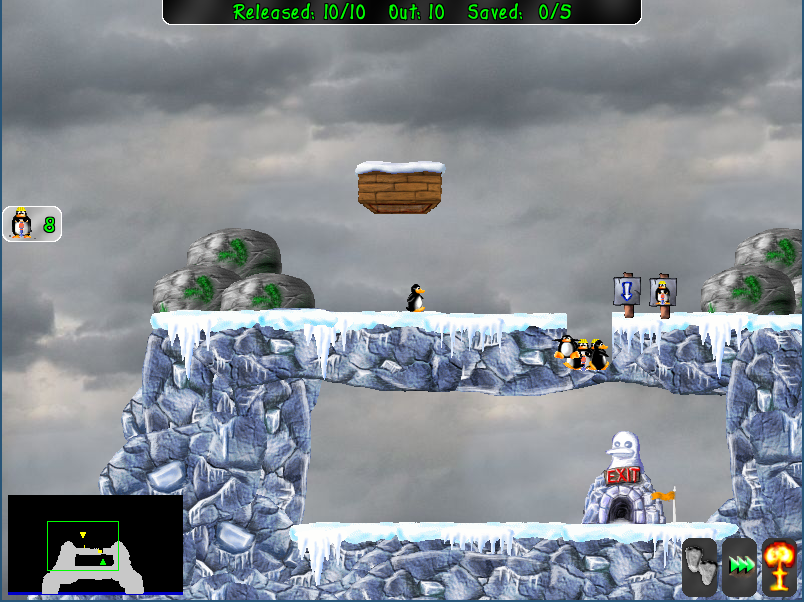
\includegraphics[width=\columnwidth]{pingus}
\caption{Pingus gameplay.
\label{fig.pingus}
}
\end{figure}

Pingus is an open-source puzzle-platform video game based on Lemmings.
The objective of the game is to guide a group of penguins through a number of
obstacles towards a designated exit (Figure~\ref{fig.pingus}).
% \footnote{Pingus gameplay video: \url{www.youtube.com/watch?v=MKrJgIFtJX0}}.
%
Pingus is developed in standard object-oriented C++, the \emph{lingua franca}
of game development \cite{games.patterns}.
The codebase%
\footnote{Pingus repository: \url{github.com/Pingus/pingus/}}
is about 40.000 lines of code (LoCs), divided into
the engine, level editor, auxiliary libraries, and the game logic itself.

According to Tim Sweeney (of Unreal Engine fame), about half the complexity in
game development resides in \emph{simulation} (aka \emph{game logic}), but
which accounts for only 10\% of the CPU budget~\cite{games.sweeney}.
%(Figure~\ref{fig.sweeney}).
%The game logic ``models the state of the game world as interacting objects
%evolve over time''.
The high development costs contrasting with the low impact on performance
appeals for alternatives with productivity in mind, especially considering that
it is the game logic that varies the most between projects.
Sweeney states that ``will gladly sacrifice 10\% of our performance for 10\%
higher productivity''.

%\begin{figure}[t]
%\centering
%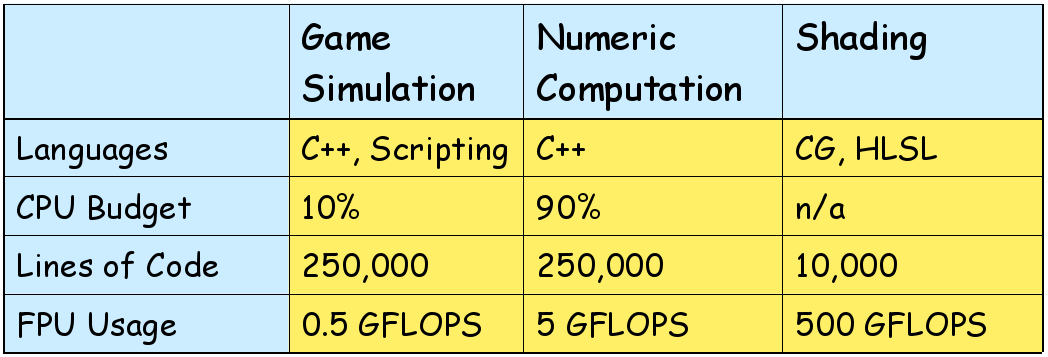
\includegraphics[width=\columnwidth]{sweeney}
%\caption{Three kinds of code~\cite{games.sweeney}.
%\label{fig.sweeney}
%}
%\end{figure}

Object-oriented games rely on the \emph{observer pattern}~\cite{games.patterns}
to handle events from the environment (e.g., key presses and timers) and also
as a notification mechanism between entities in the game logic.
%
The observers are short-lived callbacks that have to execute as fast as
possible to keep the game reactive to incoming events in real time.
%
For this reason, callbacks cannot use long-lasting locals and loops, which are
elementary capabilities of classical structured
programming~\cite{rp.deprecating,rp.rescala,sync_async.cooperative}.
%
In this sense, callbacks actually disrupt structured programming, becoming
``our generation's \code{goto}''.%
\footnote{``Callbacks as our Generations' Go To Statement'':
\url{tirania.org/blog/archive/2013/Aug-15.html}}
%\footnote{``Escape from Callback Hell'':
%\url{elm-lang.org/learn/Escape-from-Callback-Hell.elm}}

\CEU~\cite{ceu.sensys13,ceu.mod15} is a C/C++ source compatible programming
language with the following characteristics:
%
\begin{itemize}
\item \emph{Reactive}: code only executes in reactions to events.
\item \emph{Structured}: programs use structured control-flow mechanisms, such
      as \code{await} (to suspend a line of execution), and \code{par} (to
      combine multiple lines of execution).
\item \emph{Synchronous}: reactions run atomically and to completion on each
      line of execution.
      There's no implicit preemption or real parallelism, resulting in
      deterministic execution.
\end{itemize}
%
Structured reactive programming eliminates callbacks, letting programmers write
code in direct and sequential style and recover from the inversion of control
imposed by the observer pattern~\cite{rp.deprecating}.
%
\CEU provides primitives that help describing complex control-flow
relationships in the game logic more concisely.
%
\CEU supports logical parallelism with a resource-efficient implementation in
terms of memory and CPU usage~\cite{ceu.sensys13}.
The runtime is single threaded and does not rely on garbage collection.

In this work, we advocate structured synchronous reactive programming as an
expressive and productive alternative for game logic development.
We present a case study of rewriting Pingus from C++ to \CEU with the
contributions as follows:
%
\begin{itemize}
\item Alternative solutions in idiomatic \CEU with gains in productivity for
      six selected behaviors in the game logic.
\item An in-depth qualitative analysis of the proposed solutions in comparison
      to the original implementations in C++.
\item The identification of four recurrent control-flow patterns that likely
      apply to other games:
        \emph{Finite State Machines},
        \emph{Continuation Passing},
        \emph{Dispatching Hierarchies}, and
        \emph{Lifespan Hierarchies}.
        %\emph{Signaling Mechanisms}.
\end{itemize}
%
A control-flow pattern is a recurring technique to describe dependencies and
explicit orders between statements (or groups of statements) in a program.
%For instance, consider how a key press stimulus propagates through the game
%entities and also what happens with them if the stimulus causes the end of the
%game.
%
The rewriting process consisted of identifying sets of callbacks implementing
control flow in the game and translating them to \CEU using appropriate
structured constructs.
%
As an example, a double mouse click is characterized by a first click, followed
by a maximum amount of time, followed by a second click.
This behavior depends on different events (clicks and timers) which have to
occur in a particular order.
In C++, the implementation involves callbacks crossing reactions to successive
events which manipulate state variables explicitly.
%
We focus on a qualitative analysis for the programming techniques that we
applied during the rewriting process.
Not all techniques result in reduction in LoCs (especially considering the
verbose syntax of \CEU), but have other effects such as eliminating shared
variables and dependencies between classes.

The rest of the paper is organized as follows:
Section~\ref{sec.codebase} gives an overview of the Pingus codebases in C++ and
\CEU and describes our approach to identify and rewrite the control flow in the
game.
Section~\ref{sec.pats} discusses six case studies in detail which are
categorized in four control-flow patterns.
Section~\ref{sec.related} discusses related work.
Section~\ref{sec.conclusion} concludes the paper.

\section{The Pingus Codebase}
\label{sec.codebase}

\begin{figure*}[t]
\begin{verbatim}
Path              Ceu      C++   Ceu/C++    Descritpion
------------     ----     ----     ----     --------------------------------------------
game/            2064     2268     0.91     the main gameplay
  ./              710      679     1.05         main functionality
  objs/           470      478     0.98         world objects (tiles, traps, etc)
  pingu/          884     1111     0.80         pingu behaviors
    ./            343      458     0.75             main functionality
    actions/      541      653     0.83             pingu actions (bomber, climber, etc)
worldmap/         468      493     0.95     campaign worldmap
screens/         1109     1328     0.84     menus and screens
    option/       347      357     0.97         option menu
    others/       762      971     0.78         other menus and screens
misc/              56       46     1.22     miscellaneous functionality
                 ----     ----     ----
                 3697     4135     0.89
\end{verbatim}
\caption{The Pingus codebase directory tree.
\label{tab.tree}
}
\end{figure*}

In Pingus, the game logic also accounts for almost half the size of the
codebase: 18.173 from 39.362 LoCs (46\%) spread across 272 files.
%
However, about half of the game logic relates to non-reactive code, such as
dealing with configurations and options, saved games and serialization, maps
and levels descriptions, string formatting, collision detection, graph
algorithms, etc.
This part remains unchanged and relies on the integration between \CEU and
C/C++.
%
Therefore, we rewrote 9.186 LoCs spread across 126 files%
\footnote{Complete codebase: \url{github.com/an000/p/tree/master/cpp}}.
%
In order to only consider effective code in the analysis, we then removed all
headers, declarations, trivial getters \& setters, and other innocuous
statements, resulting 4.135 dense LoCs spread across 70 implementation files
originally written in C++%
\footnote{C++ codebase: \url{github.com/an000/p/tree/master/all}}.
We did the same with the implementation in \CEU, resulting in 3.697 dense LoCs%
\footnote{\CEU codebase: \url{github.com/an000/p/tree/master/all}}.
%
Figure~\ref{tab.tree} summarizes the effective codebase in the two
implementations.

Although the sections that follow compare the codebases qualitatively, the
lines with lower ratio numbers in Figure~\ref{tab.tree} correlate to the parts
of the game logic that we consider more susceptible to structured reactive
programming.
For instance, the \emph{Pingu} behavior (\emph{ratio 0.80}) contains complex
animations that are affected by timers, game rules, and user interaction.
In contrast, the \emph{Option screen} (\emph{ratio 0.97}) is a simple UI grid
with trivial mouse interactions.

As a general rewriting rule, we could identify control-flow behaviors in C++ by
looking for class members with identifiers resembling verbs, statuses, and
counters (e.g.,
\code{pressed},
\code{particle\_thrown},
\code{mode}, and
\code{delay\_count}).
Good chances are that variables with these ``suspicious names'' encode some
form of control-flow progression that cross multiple callback invocations.

We employed \emph{live code translation}, i.e., starting from the original
codebase in C++, we reimplemented piece-by-piece without breaking the game
compilation and execution.
%
This was only possible given the seamless integration between \CEU and
C/C++~\cite{ceu.sensys13}: the type systems are equivalent and the integration
happens at the source code level.
This enables trivial sharing of control and data, i.e., accessing C/C++ data
and calling C/C++ from \CEU and vice-versa.

\section{Control-Flow Patterns \& Case Studies}
\label{sec.pats}

During the course of the rewriting process, we have identified four abstract
control-flow patterns which likely apply to other games as well:

\begin{enumerate}
\item \emph{Finite State Machines}:
    Event occurrences lead to transitions between states and trigger actions
    comprising the behavior of a game entity.
\item \emph{Continuation Passing}:
    The completion of a long-lasting activity may carry a continuation in the
    game, i.e., some action to execute next.
\item \emph{Dispatching Hierarchies}:
    Entities form a dispatching hierarchy in which a container that receives a
    stimulus automatically forwards it to its managed children.
\item \emph{Lifespan Hierarchies}:
    Entities form a lifespan hierarchy in which a terminating container entity
    automatically destroys its managed children.
%\item \emph{Signaling Mechanisms}:
    %Entities often need to communicate and affect each other explicitly through
    %signaling mechanisms, especially if there is no hierarchy relationship
    %between them.
\end{enumerate}

We describe six representative game behaviors in detail distributed in the four
patterns, with their implementations in C++ and \CEU.
%
Due to space constraints, we omit five other cases and also a fifth pattern
\emph{Signaling Mechanisms} entirely.

\subsection{Finite State Machines}
\label{sec.pats.fsms}

    Event occurrences lead to transitions between states and trigger actions
    comprising the behavior of a game entity.

\subsubsection{Case Study: Detecting Double-Clicks in the \emph{Armageddon Button}}

%\begin{figure}[t]
%\centering
%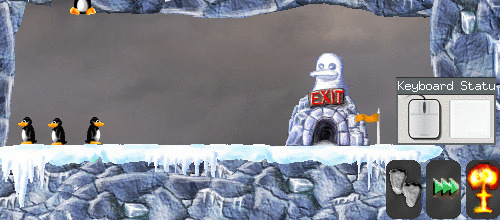
\includegraphics[width=\columnwidth]{double-click-opt}
%\caption{Double click detection.
%\label{fig.armageddon}
%}
%\end{figure}
%(Figure~\ref{fig.armageddon}).

In Pingus, a double click in the \emph{Armageddon button} at the bottom right
of the screen literally explodes all pingus.%
\footnote{Double click animation: \url{github.com/an000/p/blob/master/README.md#1} }

\begin{figure*}[t]
\begin{minipage}[t]{0.55\linewidth}
\begin{lstlisting}[numbers=left,xleftmargin=3em]
ArmageddonButton::ArmageddonButton(<...>):
    RectComponent(<...>),
    pressed(false); // button initially not pressed
    press_time(0);    // how long since 1st click?
    <...>
{
    <...>
}

void ArmageddonButton::draw (<...>) {
    <...>
}

void ArmageddonButton::update (float delta) {
    <...>
    if (pressed) {
        press_time += delta;
        if (press_time > 1.0f) {
            pressed = false; // give up, 1st click
            press_time = 0;  // was too long ago
        }
    } else {
        <...>
        press_time = 0;
    }
}

void ArmageddonButton::on_click (<...>) {
    if (pressed) {
        send_armageddon_event();
    } else {
        pressed = true;
    }
}
\end{lstlisting}
\centering\small{\ax Implementation in C++}
\end{minipage}
%
\begin{minipage}[t]{0.45\linewidth}
\begin{lstlisting}[numbers=left,xleftmargin=3em]
do
    var RectComponent r = <...>;
    <...>
    loop do
        await r.on_click;
        watching 1s do
            await r.on_click;
            break;
        end
    end
    <...>
    emit game.armageddon;
end




















.
\end{lstlisting}
\centering\small{\bx Implementation in \CEU}
\end{minipage}
%\rule{8.4cm}{0.37pt}
\caption{ Detecting double-clicks in the \emph{Armageddon button}.
\label{lst.armageddon}
}
\end{figure*}

Figure~\ref{lst.armageddon}.a shows the C++ implementation for the class
\code{ArmageddonButton} with methods for rendering the button and handling
mouse and timer events.
The code focus on the double click detection and hides unrelated parts with
\code{<...>}.
%
The methods \code{update} (ln. 14--26) and \code{on\_click} (ln. 28--34) are
examples of \emph{short-lived callbacks}, which are pieces of code that execute
atomically in reaction to external input events.
The callback \code{on\_click} reacts to mouse clicks detected by the base class
\code{RectComponent} (ln. 2), while the callback \code{update} continuously
reacts to the passage of time, frame by frame.
%Callbacks are short lived because they must react to input as fast as possible
%to let other callbacks execute, keeping the game with real-time responsiveness.
%
The class first initializes the variable \code{pressed} (ln. 3) to track the
first click (ln. 32).
It also initializes the variable \code{press\_time} (ln. 4) to count the time
since the first click (ln. 16--17).
If another click occurs within 1 second, the class signals the double click to
the application (ln. 29--30).
Otherwise, the \code{pressed} and \code{press\_time} state variables are reset
(ln. 18--21). 
%
Figure~\ref{fig.armageddon.fsm} illustrates how we can model the double-click 
behavior in C++ as a state machine.
The circles represent the state of the variables in the class, while the arrows 
represent the callbacks manipulating state.
%
Note in the code how the accesses to the state variables are spread
across the entire class.
For instance, the distance between the initialization of \code{pressed} (ln.
3) and the last access to it (ln. 32) is over 40 lines in the original file.
Arguably, this dispersion of code across methods makes the understanding and 
maintenance of the double-click behavior more difficult.
Also, even though the state variables are private, unrelated methods such as 
\code{draw}, which is defined in middle of the class (ln. 10--12), can
potentially access them.

\begin{figure}[t]
\centering
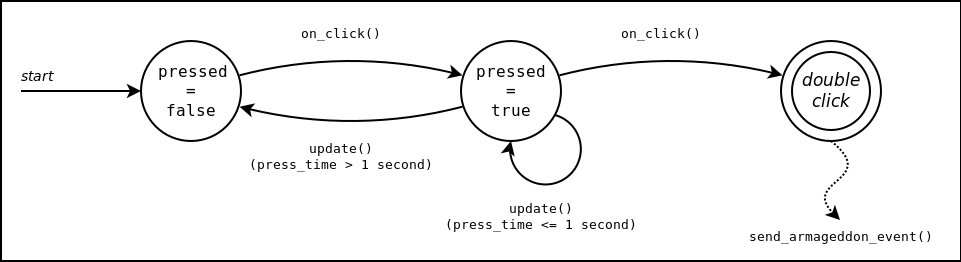
\includegraphics[width=\columnwidth]{double-click}
\caption{State machine for detecting double-clicks in the
         \emph{Armageddon button}.
\label{fig.armageddon.fsm}
}
\end{figure}

\CEU provides structured constructs to deal with events, aiming to eradicate
explicit manipulation of state variables for control-flow purposes.
%
In Figure~\ref{lst.armageddon}.b, the loop to detect double clicks (ln. 4--10)
awaits the first click (ln. 5) and then, while watching 1 second (ln. 6--9),
awaits the second click (ln. 7).
If the second click occurs within 1 second, the \code{break} terminates the
loop (ln. 8) and the \code{emit} in sequence signals the double click to the
application (ln. 12).
Otherwise, the \code{watching} block as a whole aborts after 1 second  and the
loop restarts, falling back to the first click \code{await} (ln. 5).
%
Double click detection in \CEU doesn't require state variables and is entirely
self-contained in the \code{loop} body.
Also, these 7 lines of code \emph{only} detect the double click, leaving the
actual effect to happen outside the loop (ln. 12) as well as all unrelated
code such as redrawing the button.

\subsubsection{Case Study: The \emph{Bomber Action} Animation Sequence}
\label{sec.pats.fsms.2}

%\begin{figure}[t]
%\centering
%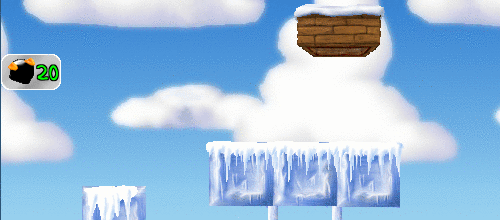
\includegraphics[width=\columnwidth]{bomber-anim}
%\caption{ The \emph{Bomber action}.
%\label{fig.bomber.anim}
%}
%\end{figure}

\begin{figure}[t]
\centering
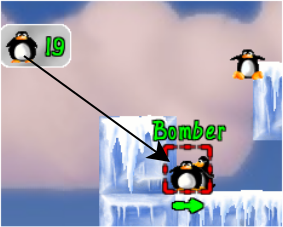
\includegraphics[width=120px]{bomber-01}
\caption{ Assigning the \emph{Bomber action} to a pingu.
\label{fig.bomber.action}
}
\end{figure}

\begin{figure}[t]
\centering
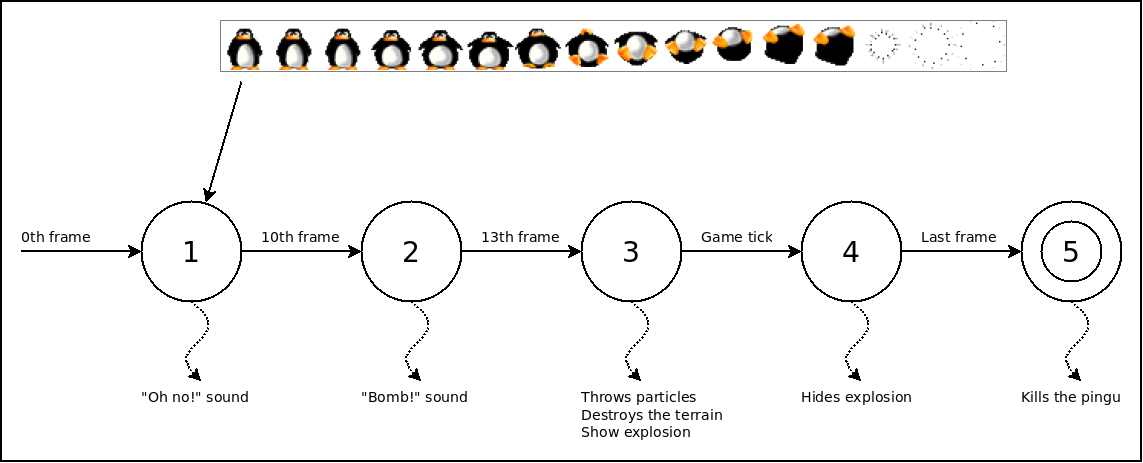
\includegraphics[width=\columnwidth]{bomber-state}
\caption{ State machine for the \emph{Bomber animation} sequence.
\label{fig.bomber.fsm}
}
\end{figure}

\begin{figure*}[th!]
\begin{minipage}[t]{0.50\linewidth}
\begin{lstlisting}[numbers=left,xleftmargin=3em]
Bomber::Bomber (Pingu* p) :
  <...>
  sprite(<...>),          // bomber sprite
  sound_played(false),    // tracks state 2
  particle_thrown(false), // tracks state 3
  colmap_exploded(false), // tracks state 3
  gfx_exploded(false)     // tracks state 4
{
  <...>
  // 1. plays a "Oh no!" sound.
  play_sound("ohno");
}

void Bomber::update () {
  sprite.update();
  <...>   // pingu movement

  // 2. plays a "Bomb!" sound.
  if (sprite.frame()==10 && !sound_played) {
    sound_played = true;
    play_sound("plop");
  }

  // 3. particles, terrain, explosion sprite
  if (sprite.frame()==13 && !particle_thrown) {
    particle_thrown = true;
    get_world()->get_particles()->add(...);
  }
  if (sprite.frame()==13 && !colmap_exploded) {
    colmap_exploded = true;
    get_world()->remove(bomber_radius, <...>);
  }

  // 5. kills the Pingu
  if (sprite.is_finished ()) {
    pingu->set_status(PS_DEAD);
  }
}

void Bomber::draw (SceneContext& gc) {
  // 3. particles, terrain, explosion sprite
  // 4. tick: hides the explosion sprite
  if (sprite.frame()==13 && !gfx_exploded) {
    gfx_exploded = true;
    gc.color().draw(explo_surf, <...>);
  }
  gc.color().draw(sprite, pingu->get_pos());
}
\end{lstlisting}
\centering\small{\ax Implementation in C++}
\end{minipage}
%
\begin{minipage}[t]{0.50\linewidth}
\begin{lstlisting}[numbers=left,xleftmargin=3em]
code/await Bomber (void) -> ActionName
do
  <...>
  spawn Mover();  // movement in the background
  var Sprite s = spawn Sprite(<...>);
                  // animation in the background
  watching s do
    // 1. plays a "Oh no!" sound.
    {play_sound("ohno")};

    // 2. plays a "Bomb!" sound.
    await game.update until s.sprite.frame == 10;
    {play_sound("plop")};

    // 3. particles, terrain, explosion sprite
    await game.update until s.sprite.frame == 13;
    spawn PinguParticles(<...>) in particles;
    call Game_Remove({&bomber_radius}, <...>);
    do
      <...>
      spawn Sprite(<...>);      // explosion

      // 4. tick: hides the explosion sprite
      await game.update;
    end
    await FOREVER;
  end

  // 5. kills the pingu
  escape DEAD;
end
















.
\end{lstlisting}
\centering\small{\bx Implementation in \CEU}
\end{minipage}
%\rule{8.4cm}{0.37pt}
\caption{ The \emph{Bomber action} sequence.
\label{lst.bomber}
}
\end{figure*}

In Pingus, the player may assign actions to specific pingus, as illustrated in
Figure~\ref{fig.bomber.action}.
%
The \emph{Bomber action} explodes the clicked pingu, throwing particles around
and also destroying the terrain under its radius.%
\footnote{Bomber action animation: \url{github.com/an000/p/blob/master/README.md#2} }
%
We can model the explosion animation with a sequential state machine
(Figure~\ref{fig.bomber.fsm}) with effects associated to specific frames as
follows%
\footnote{State machine animation: \url{github.com/an000/p/blob/master/README.md#3} }:
%
\begin{enumerate}
\item 0th frame:  plays a "Oh no!" sound.
\item 10th frame: plays a "Bomb!" sound.
\item 13th frame: throws particles, destroys the terrain, and shows an
                  explosion sprite.
\item Game tick:  hides the explosion sprite.
\item Last frame: kills the pingu.
\end{enumerate}

In C++, the class \code{Bomber} in Figure~\ref{lst.bomber}.a defines the
callbacks \code{draw} and \code{update} to manage the state machine described
above.
%
The class first defines one state variable for each effect to perform
(ln. 4--7).
The ``Oh no!'' sound plays as soon as the object starts in \emph{state-1} 
(ln. 11).
The \code{update} callback (ln. 14--38) first updates the pingu animation and
movement on every frame regardless of its current state (ln. 15--16).
When the animation reaches the 10th frame, it plays the ``Bomb!'' sound and 
switches to \emph{state-2} (ln. 18--22).
The state variable \code{sound\_played} is required because the sprite frame
doesn't necessarily advance on every \code{update} invocation (e.g.,
\code{update} may execute twice during the 10th frame).
The same reasoning and technique applies to \emph{state-3} (ln. 24--32 and
43--44).
The explosion sprite appears in a single frame in \emph{state-4} (ln. 45).
Finally, the pingu dies after the animation frames terminate (ln. 34--37).
%
Note that a single numeric state variable suffices to track the states, but the
original authors probably chose to encode each state in an independent boolean 
variable to rearrange and experiment with them during development.
Still, due to the short-lived nature of callbacks, state variables are 
unavoidable and are actually the essence of object-oriented programming
(i.e., \emph{methods with mutable state}).
%
Like double click detection in C++, note that the state machine is encoded
across 3 different methods, each intermixing code with unrelated functionality
(e.g., changing frames, moving, and redrawing).

The equivalent code in \CEU for the \emph{Bomber action} in
Figure~\ref{lst.bomber}.b does not use state variables and reflects the
sequential state machine implicitly, using \code{await} statements in direct
style to separate the effects.
%
The \code{Bomber} is a \code{code/await} abstraction of \CEU, which is similar
to a coroutine or fiber~\cite{sync_async.cooperative}: a subroutine that
retains runtime state, such as local variables and the program counter, across
reactions to events (i.e., across \code{await} statements).
The pingu movement and sprite animation are isolated in two other
\code{code/await} abstractions and execute in separate through the \code{spawn}
primitive (ln. 4--5).
The event \code{game.update} (ln. 12,16,24) is analogous to the \code{update}
callback of C++ and occurs on every frame.
%
The code tracks the animation aliveness (ln. 7--27) and, on termination,
performs the last bomber effect, killing the pingu (ln. 30).
As soon as the animation starts, the code performs the first effect (ln. 9).
The intermediate effects are performed when the corresponding conditions occur
(ln. 12,16,24).
The \code{do-end} block (ln. 19--25), restricts the lifespan of the
single-frame explosion sprite (ln. 21): after the next game tick (ln. 24), the
block terminates and automatically destroys the spawned abstraction (removing
it from the screen).
%
In contrast with the implementation in C++, all effects occur in a contiguous
chunk of code (ln. 7--30), which handles no extra functionality.

\subsubsection{Summary \& Uses in Pingus}

The structured constructs of \CEU introduce some advantages in comparison to 
explicit state machines:
%
\begin{itemize}
\item They encode all states with direct sequential code, eliminating shared
      state variables.
\item They handle all states (and only them) in the same contiguous block,
      improving code encapsulation.
\end{itemize}
%
Object-oriented games also adopt the \emph{state pattern} to model state
machines with subclasses describing each possible state~\cite{games.patterns}.
However, this approach is not fundamentally different from Pingus' use of
\code{switch} or \code{if} branches for each possible state.

\begin{figure}[t]
\begin{verbatim}
Action       Ceu    C++   Explicit State
---------   ----   ----   -----------------
Bomber        23     50   4 state variables
Bridger       75    100   2 state variables
Drown          6     15   1 state variable
Exiter         7     22   2 state variables
Splashed       6     19   2 state variables
\end{verbatim}
\caption{Pingus actions in \CEU and C++.
\label{tab.actions}
}
\end{figure}

Pingus supports 16 actions in the game.
As Figure~\ref{tab.actions} shows, 5 of them implement at least one state
machine and are considerable smaller in \CEU in terms of LoCs after eliminating
the state variables.
%
Considering the other 11 actions, the reduction in LoCs is negligible.
This asymmetry in the implementation of actions illustrates the gains in
expressiveness when describing state machines in direct style.

%As other examples, detecting mouse dragging in the scenario and in the small
%map to move the game viewport also involves state machines.
%State machines also appear in the \emph{FPS counter} and in UI widgets with
%visual feedback.

Among the 65 implementation files in \CEU, we found 29 cases in 25 files using
structured mechanisms to substitute states machines.
They manifest as \code{await} statements in sequence or in aborting constructs
such as \code{par/or} and \code{watching}.

\subsection{Continuation Passing}
\label{sec.pats.cps}

    The completion of a long-lasting activity may carry a continuation in the
    game, i.e., some action to execute next.

\subsubsection{ Transition to the \emph{Credits Screen} from the \emph{Story Screen} }

\begin{figure*}[t]
\begin{minipage}[t]{0.50\linewidth}
\begin{lstlisting}[numbers=left,xleftmargin=3em]
StoryDot::StoryDot(const FileReader& reader) :
  credits(false), // do not display by default
{
  <...>
  reader.read("credits", credits); // from file
}

void StoryDot::on_click() {
  <...>
  push_screen(<StoryScreen>(<...>, credits));
  <...>
}

///

StoryScreenComp::StoryScreenComp (<...>) :
  credits(credits),
  <...>
{
  <...>
}

<...>   // draw and update page

void StoryScreenComp::next_text() {
  if (!displayed) {
    <...>
  } else {
    <...>
    if (!pages.empty()) {
      <...>
    } else {
      if (credits) {
        replace_screen(<Credits>(<...>));
      } else {
        pop_screen();
      }
    }
  }
}
\end{lstlisting}
\centering\small{\ax Implementation in C++}
\end{minipage}
%
\begin{minipage}[t]{0.50\linewidth}
\begin{lstlisting}[numbers=left,xleftmargin=3em]
loop do
  var int ret = await Worldmap();
  if ret=={STORY_MAP} or ret=={STORY_CREDITS} then
    <...>
    var bool is_click = await Story();
    if is_click and ret=={STORY_CREDITS} then
      <...>
      await Credits();
    end
  else
    <...>
  end
end


























.
\end{lstlisting}
\centering\small{\bx Implementation in \CEU}
\end{minipage}
%\rule{8.4cm}{0.37pt}
\caption{ Transition from \emph{Story} to \emph{Credits screen}.
\label{lst.story}
}
\end{figure*}

The campaign world map has clickable blue dots for introductory and ending
ambience stories in the two extremes of the map progress trail.
For introductory stories, the game returns to the world map after displaying 
the story pages.
For ending stories, the game also displays a \emph{Credits screen} before
returning to the world map.%
\footnote{Story screen animation: \url{github.com/an000/p/blob/master/README.md#4} }

In C++, the class \code{StoryDot} in Figure~\ref{lst.story}.a (ln. 1--12) reads
the level file (ln. 5) to check whether its an ending story and should, after
termination, display the \emph{Credits screen}.
%
The boolean variable \code{credits} is passed to the class
\code{StoryScreen} (ln. 10) and represents the screen continuation, i.e., what
to do after displaying the story.
The class \code{StoryScreen} (not shown) then forwards the continuation even
further to the auxiliary class \code{StoryScreenComp} (ln. 16--40).
%
When the method \code{next\_text} has no pages left to display (ln. 32--38),
it decides where to go next, depending on the continuation flag
\code{credits} (ln. 33--37).

In \CEU, the \code{loop} of Figure~\ref{lst.story}.b controls the flow between
the screens to display as a direct sequence of statements.
%
We first invoke the \code{Worldmap} (ln. 2), which exhibits the map and let
the player interact with it until a dot is clicked.
If the player selects a story dot (ln. 4--9), we invoke the \code{Story}
and await its termination (ln. 5).
Finally, we check the returned values (ln. 6) to perhaps display the
\code{Credits} screen (ln. 8).
The enclosing loop restores the \code{Worldmap} and repeats the process.

\begin{figure}[t]
\centering
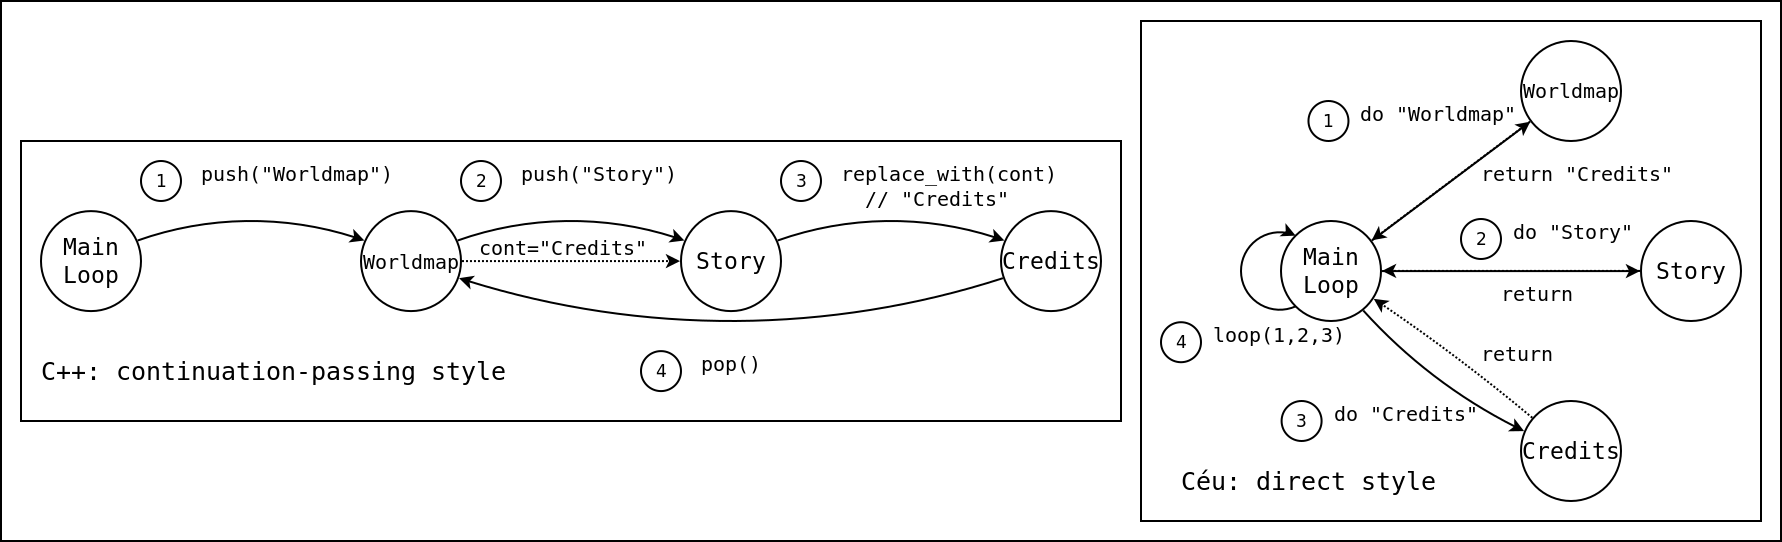
\includegraphics[width=\columnwidth]{continuation}
\caption{ Continuation (C++) vs Direct (\CEU) Styles.
\label{fig.story}
}
\end{figure}

Figure~\ref{fig.story} illustrates the \emph{continuation-passing style} of
C++ and the \emph{direct style} of \CEU for screen transitions:

\begin{enumerate}
\item \code{Main Loop} $\longrightarrow$ \code{Worldmap}:
    \begin{itemize}
    \item C++ uses an explicit stack to push the \code{Worldmap} screen.
    \item \CEU invokes the \code{WorldMap} screen expecting a return value
          (ln. 2).
    \end{itemize}
\item \code{Worldmap} (\emph{blue dot click}) $\longrightarrow$ \code{Story}:
    \begin{itemize}
    \item C++ pushes the \code{Story} screen passing the continuation flag
          (ln. 10).
    \item \CEU stores the \code{Worldmap} return value and invokes the \code{Story} screen
          (ln. 2,5).
    \end{itemize}
\item \code{Story} $\longrightarrow$ \code{Credits}:
    \begin{itemize}
    \item C++ replaces the current \code{Story} screen with the \code{Credits}
          screen (ln. 34).
    \item \CEU invokes the \code{Credits} screen after the \code{await Story}
          returns (ln. 8).
    \end{itemize}
\item \code{Credits} $\longrightarrow$ \code{Worldmap}:
    \begin{itemize}
    \item C++ pops the \code{Credits} screen, going back to the \code{Worldmap}
          screen.
          \CEU uses an enclosing \code{loop} to restart the process (ln. 1--13).
    \end{itemize}
\end{enumerate}

In contrast with C++, the screens in \CEU are decoupled and only the
\code{Main Loop} touches them: the \code{Worldmap} has no references to
\code{Story}, which has no references to \code{Credits}.

\subsubsection{Summary \& Uses in Pingus}

The direct style of \CEU has some advantages in comparison to the 
continuation-passing style:
%
\begin{itemize}
\item It uses structured control flow (i.e., sequences and loops) instead of 
      explicit data structures (e.g., stacks) and continuation variables (e.g.
      boolean flags).
\item The activities in sequence are decoupled and do not hold references to
      one another. % TODO: esta no outro exemplo
\item A single parent class describes the flow between the activities in a 
      self-contained block of code. % TODO: esta no outro exemplo
\end{itemize}

Continuation passing typically controls the overall structure of the game,
such as screen transitions in menus and level progressions.
%
\CEU uses the direct style techniques in five cases involving screen
transitions:
the main menu, the level menu, the level set menu, the world map loop, and
the gameplay loop.
%
It also uses the same technique for the loop that switches the pingu actions
during gameplay.

\subsection{Dispatching Hierarchies}
\label{sec.pats.dispatching}

    Entities form a dispatching hierarchy in which a container that receives a
    stimulus automatically forwards it to its managed children.

\subsubsection{Case Study: \emph{Bomber Action} \Code{draw} and \Code{update} Dispatching}

\begin{figure}[t]
\centering
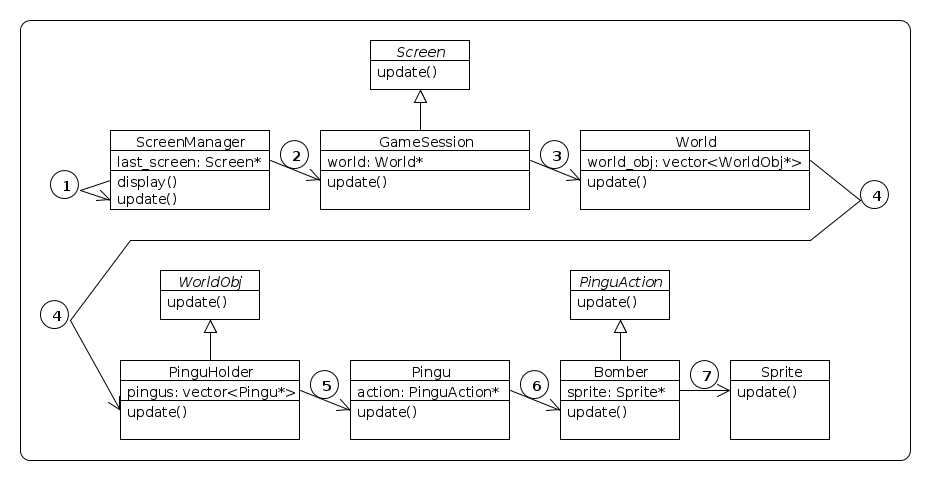
\includegraphics[width=\columnwidth]{hierarchy}
\caption{Dispatching chain for \code{update}.
\label{fig.hier}
}
\end{figure}

\begin{figure*}[t]
\begin{minipage}[t]{0.50\linewidth}
\begin{lstlisting}[numbers=left,xleftmargin=3em]
class Bomber : public PinguAction {
    <...>
    Sprite sprite;
}

Bomber::Bomber (<...>) : <...> {
    sprite.load(<...>);
    <...>
}

void Bomber::update () {
    sprite.update();
}

void Bomber::draw (SceneContext& gc) {
    <...>
    gc.color().draw(sprite, <...>);
}
\end{lstlisting}
\centering\small{\ax Implementation in C++}
\end{minipage}
%
\begin{minipage}[t]{0.50\linewidth}
\begin{lstlisting}[numbers=left,xleftmargin=3em]
code/await Bomber (void) -> ActionName do
    <...>
    var Sprite sprite = spawn Sprite(<...>);
    <...>
end












.
\end{lstlisting}
\centering\small{\bx Implementation in \CEU}
\end{minipage}
%\rule{8.4cm}{0.37pt}
\caption{ \emph{Bomber action} \code{draw} and \code{update} dispatching.
\label{lst.hier}
}
\end{figure*}

TODO: code for Sprite update?

In C++, the class \code{Bomber} presented in Figure~\ref{lst.hier}.a declares a
\code{sprite} member (ln. 3) to handle its animation frames
(Figure~\ref{fig.bomber.fsm}).
%
The \code{Sprite} class is part of the game engine and knows how to update and
render itself.
However, the \code{Bomber} still has to respond to \code{update} and
\code{draw} requests from the game and forward them to the sprite
(ln. 11--13 and 15--18).
%
To understand how the \code{update} callback flows from the original
environment stimulus to the game down to the sprite, we need to follow a long
chain of 7 method dispatches (Figure~\ref{fig.hier}):
%
\begin{enumerate}
\item \code{ScreenManager::display} in the main game loop calls \code{update}.
\item \code{ScreenManager::update} calls \code{last\_screen->update} for the
      active game screen (a \code{GameSession} instance, considering the
      \code{Bomber}).
\item \code{GameSession::update} calls \code{world->update}.
\item \code{World::update} calls \code{obj->update} for each object in the
      world.
\item \code{PinguHolder::update} calls \code{pingu->update} for each pingu
      alive.
\item \code{Pingu::update} calls \code{action->update} for the active pingu
      action.
\item \code{Bomber::update} calls \code{sprite.update}.
      \code{Sprite::update} finally updates the animation frame.
\end{enumerate}
%
Each dispatching step in the chain is necessary considering the game
architecture:
%
\begin{itemize}
\item With a single assignment to \code{last\_screen}, we can easily deactivate
      the current screen and redirect all dispatches to a new screen (step 2).
\item The \code{World} class manages and dispatches events to all game
      entities, such as all pingus and traps, with the common interface
      \code{WorldObj} (step 4).
\item Since it is common to iterate only over the pingus (vs. all world
      objects), the container \code{PinguHolder} manages all pingus (step 5).
\item Since a single pingu can change between actions during lifetime, the
      \code{action} member decouples them with another level of indirection
      (step 6).
\item Sprites are part of the game engine and are reusable everywhere (e.g., UI
      buttons, world objects, etc.), so it is also convenient to decouple them
      from actions (step 7).
\end{itemize}
%
The \code{draw} callback flows through the same dispatching hierarchy until
reaching the \code{Sprite} class.

In \CEU, the \code{Bomber} abstraction presented in Figure~\ref{lst.hier}.b
spawns a \code{Sprite} animation instance on its body (ln. 3).
%
The \code{Sprite} abstraction can react directly to external \code{update}
and \code{draw} events, bypassing the program hierarchy entirely.
External events in \CEU are broadcasted to the entire application.
While (\emph{and only while}) the bomber abstraction is alive, the sprite
animation remains alive.
The radical decoupling between the program hierarchy and reactions to events
eliminates dispatching chains entirely.
Note that one can still declare a local event and restrict its visibility like
a local variable.

\subsubsection{Summary \& Uses in Pingus}

Passive entities subjected to hierarchies require a dispatching architecture
that makes the reasoning about the program harder:

\begin{itemize}
\item The full dispatching chain may go through dozens of files.
\item The dispatching chain may interleave between classes specific to the game
      and also classes from the game engine (possibly third-party classes).
\end{itemize}

In C++, the update subsystem touches 39 files with around 100 lines of code
just to forward \code{update} methods through the dispatching hierarchy.
For the drawing subsystem, 50 files with around 300 lines of code.
The implementation in C++ also relies on dispatching hierarchy for
\code{resize} callbacks, touching 12 files with around 100 lines of code.
%
Most of this code is eliminated in \CEU since abstractions can react directly
to the environment, not depending on hierarchies spread across multiple files.

Note that dispatching hierarchies cross game engine code, suggesting that most
games also rely heavily on this control-flow pattern.
In the case of the Pingus engine, we rewrote 9 files from C++ to \CEU, reducing
them from 515 to 173 LoCs (not shown in Figure~\ref{tab.tree}), mostly due to
dispatching code removal.

\subsection{Lifespan Hierarchies}
\label{sec.pats.lifespan}

    Entities form a lifespan hierarchy in which a terminating container entity
    automatically destroys its managed children.

\subsubsection{Case Study: Game UI Widgets}

\begin{figure}[t]
\centering
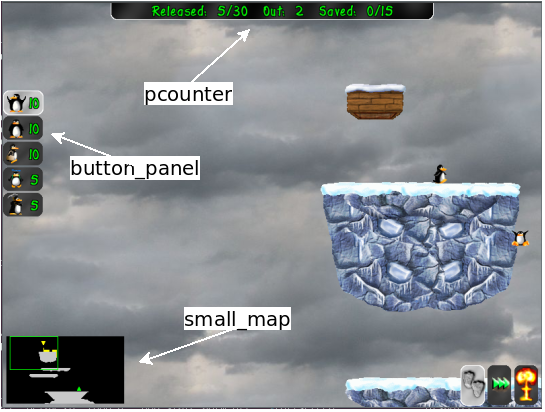
\includegraphics[width=\columnwidth]{game-session-arrows}
\caption{UI children with static lifespan.
\label{fig.ui}
}
\end{figure}

\begin{figure*}[t]
\begin{minipage}[t]{0.54\linewidth}
\begin{lstlisting}[numbers=left,xleftmargin=3em]
GameSession::GameSession(<...>) :
    <...>
{
    <...>      // these widgets are always active...
    btpanel  = new ButtonPanel(<...>);
    pcounter = new PingusCounter(<...>);
    smallmap = new SmallMap(<...>);
    <...>
    uimgr->add(btpanel);  // ...but are added
    uimgr->add(pcounter); //  dynamically to the
    uimgr->add(smallmap); //  dispatching hierarchy
    <...>
}
\end{lstlisting}
\centering\small{\ax Implementation in C++}
\end{minipage}
%
\begin{minipage}[t]{0.46\linewidth}
\begin{lstlisting}[numbers=left,xleftmargin=3em]
code/await Game (void) do
    <...> // other coexisting functionality
    spawn ButtonPanel(<...>);
    spawn PingusCounter(<...>);
    spawn SmallMap(<...>);
    <...> // other coexisting functionality
end





.
\end{lstlisting}
\centering\small{\bx Implementation in \CEU}
\end{minipage}
%\rule{8.4cm}{0.37pt}
\caption{ Managing the UI widgets lifecycle.
\label{lst.ui}
}
\end{figure*}

Figure~\ref{fig.ui} shows the game UI widgets with the action buttons, score
counters, and a small map which all coexist with the game screen during its
whole lifespan.

In C++, the widgets are created in the constructor of the class
\code{GameSession} in Figure~\ref{lst.ui}.a (ln. 5--7), added to a UI container
(ln. 9--11), and are never removed since they must always be visible.
Arguably, to better express the intent of making them coexist with the game
screen, the widgets could alternatively be declared as top-level automatic
(non-dynamic) members.
However, the class relies on a container to automate \code{draw} and
\code{update} dispatching to the widgets, as discussed in
Section~\ref{sec.pats.dispatching}.
The container method \code{add} expects only dynamically allocated children
because they are automatically deallocated inside the container destructor.
%
However, the dynamic nature of containers in C++ demand extra caution from
programmers:
%
\begin{itemize}
\item When containers are part of a dispatching chain, it gets even harder to
      know which objects are dispatched at a given moment:
      one has to ``simulate'' the program execution and track calls to
      \code{add} and \code{remove}.
\item For objects with dynamic lifespan, calls to \code{add} must always have
      matching calls to \code{remove}:
      missing calls to \code{remove} lead to memory and CPU leaks (to be
      discussed as the \emph{lapsed listener} problem in
      Section~\ref{sec.pats.lifespan.2}).
\end{itemize}

In \CEU, the UI entities that coexist just have to be created in the same
lexical block in Figure~\ref{lst.ui}.b (ln. 3--5).
%
Since abstractions can react independently, they do not require a dispatching
container.
%
Lexical lifespan never requires containers, allocation and deallocation, or
explicit references.
In addition, all required memory is known at compile time, similarly to
stack-allocated local variables.
%
The \emph{Bomber action} of Section~\ref{sec.pats.fsms.2} also relies on
lexical scope to delimit the lifespan of the explosion sprite to a single
frame (Figure~\ref{lst.bomber}, ln. 19--25).

\subsubsection{Case Study: Managing the Pingus Lifecycle}
\label{sec.pats.lifespan.2}

%\begin{figure}[t]
%\centering
%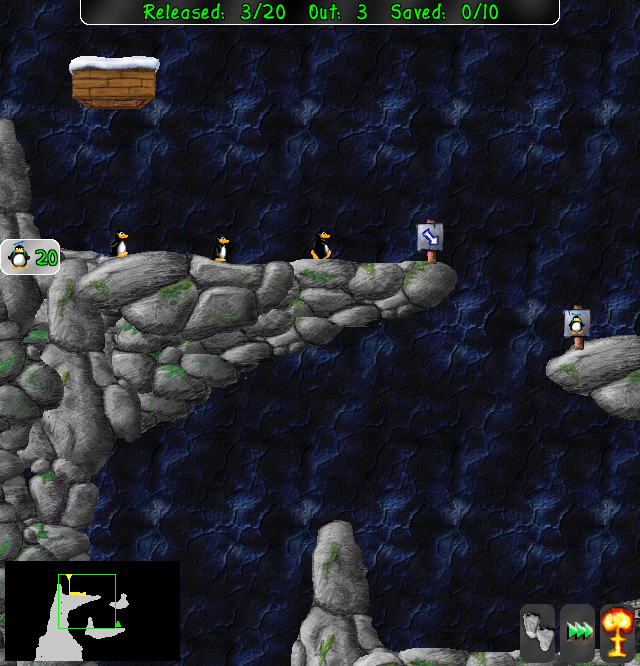
\includegraphics[width=\columnwidth]{pingus_create_die-anim}
%\caption{Creation and death of pingus.
%\label{fig.pingus_create_die}
%}
%\end{figure}

A pingu is a dynamic entity created periodically and destroyed under certain
conditions, such as falling from a high altitude%
\footnote{Death of pingus animation: \url{github.com/an000/p/blob/master/README.md#5} }.
%

\begin{figure*}[t]
\begin{minipage}[t]{0.50\linewidth}
\begin{lstlisting}[numbers=left,xleftmargin=3em]
Pingu* PinguHolder::create_pingu (<...>) {
    <...>
    Pingu* pingu = new Pingu (<...>);
    pingus.push_back(pingu);
    <...>
}

void PinguHolder::update() {
    <...>
    while(pingu != pingus.end()) {
        (*pingu)->update();
        if ((*pingu)->get_status() == PS_DEAD) {
            pingu = pingus.erase(pingu);
        }
        <...>
        ++pingu;
    }
}

.
\end{lstlisting}
\centering\small{\ax Implementation in C++}
\end{minipage}
%
\begin{minipage}[t]{0.50\linewidth}
\begin{lstlisting}[numbers=left,xleftmargin=3em]
code/await Game (void) do
    <...>
    pool[] Pingu pingus;
    code/await Pingu_Spawn (<...>) do
        <...>
        spawn Pingu(<...>) in pingus;
    end
    <...>   // code invoking Pingu_Spawn
end

code/await Pingu (<...>) do
    <...>
    loop do
        await game.update;
        if Pingu_Is_Out_Of_Screen() then
            <...>
            escape {PS_DEAD};
        end
    end
end
\end{lstlisting}
\centering\small{\bx Implementation in \CEU}
\end{minipage}
%\rule{8.4cm}{0.37pt}
\caption{ Managing the pingus lifecycle.
\label{lst.pingus}
}
\end{figure*}

In C++, the class \code{PinguHolder} in Figure~\ref{lst.pingus}.a is a
container that holds all alive pingus.
%
The method \code{PinguHolder::create\_pingu} (ln. 1--6) is called periodically
to create a new \code{Pingu} and add it to the \code{pingus} collection
(ln. 3--4).
The method \code{PinguHolder::update} (ln. 8--18) checks the state of all
pingus on every frame, removing those with the dead status (ln. 12--14).
%
Entities with dynamic lifespan in C++ require explicit \code{add} and
\code{remove} calls associated to a container (ln. 4,13).
Without the \code{erase} call above, a dead pingu would remain in the
collection still with updates on every frame (ln. 11).
Since the \code{draw} behavior for a dead pingu is innocuous, the death could
go unnoticed when testing it but the program would keep consuming memory and
CPU time.
This problem is known as the \emph{lapsed listener}~\cite{games.patterns} and
also occurs in languages with garbage collection:
a container typically holds a strong reference to a child (sometimes the only 
reference to it), and the runtime cannot magically detect it as garbage.

\begin{figure}[t]
\centering
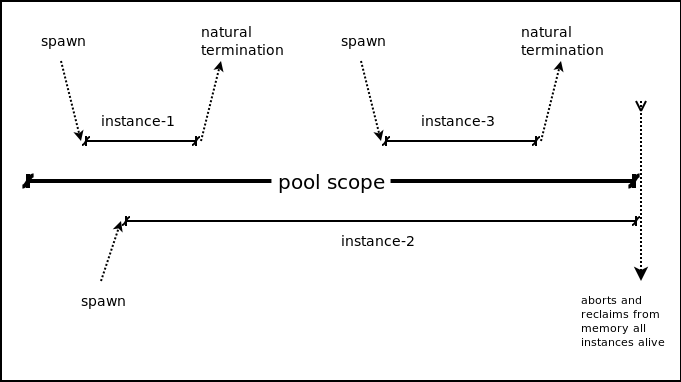
\includegraphics[width=\columnwidth]{pool}
\caption{Lifespan of dynamic instances.
\label{fig.pool}
}
\end{figure}

\CEU supports \code{pool} declarations to hold dynamic abstraction instances.
Additionally, the \code{spawn} statement supports a pool identifier to
associate the new instance with a pool.
%
The game screen in Figure~\ref{lst.pingus}.b spawns a new \code{Pingu} on every
invocation of \code{Pingu\_Spawn} (ln. 4--7).
%
The \code{spawn} statement (ln. 6) specifies the pool declared at the top-level
block of the game screen (ln. 3).
In this case, the lifespan of the new instances follows the scope of the pool
(ln. 1--9) instead of the enclosing scope of the \code{spawn} statement
(ln. 4--7).
Since pools are also subject to lexical scope, the lifespan of all dynamically
allocated pingus is constrained to the game screen.
%
Lexical scopes handle memory and event dispatching automatically for static
instances and also for pools.
However, the lifespan of a dynamic instance does not necessarily have to match
the lifespan of its associated pool (Figure~\ref{fig.pool}).
In \CEU, when the execution block of a dynamic instance terminates, which
characterizes its \emph{natural termination}, the instance is automatically
removed from its pool.
Therefore, dynamic instances do not require any extra bookkeeping related to 
containers or explicit deallocation.
%
To remove a pingu from the game in \CEU, we just need to terminate its execution
block according to the appropriate conditions:
%
The \code{escape} statement (ln. 17) aborts the execution block of the
\code{Pingu} instance, removing it from its associated pool automatically.
Hence, a dynamic instance that terminates naturally leaves no traces in the 
program.

\subsubsection{Summary \& Uses in Pingus}

Lexical lifespan for static instances and natural termination for dynamic
instances provide some advantages in comparison to lifespan hierarchies through
containers:

\begin{itemize}
\item Lexical scope makes an abstraction lifespan explicit in the source code.
      All entities in a game have an associated lexical lifespan.
\item The memory for static instances is known at compile time.
\item Natural termination makes an instance innocuous and, hence, susceptible
      to immediate reclamation.
\item Abstraction instances (static or dynamic) never require explicit
      manipulation of pointers/references.
\end{itemize}

The implementation in \CEU has over 200 static instantiations spread across all
65 files.
For dynamic entities, it defines 23 pools in 10 files, with almost 96
instantiations across 37 files.
Pools are used to hold explosion particles, levels and level sets from files,
gameplay \& worldmap objects, and UI widgets.

\section{Related Work}
\label{sec.related}

The control-flow patterns closely relate to the \emph{GoF} behavioral
patterns~\cite{gof}, which some previous work discuss in the context of video
games~\cite{games.patterns,games.gof.2015,games.gof.2007}.
%
The original Pingus in C++ uses variations of the
    \emph{state} (Sections~\ref{sec.pats.fsms}~and~\ref{sec.pats.cps}),
    \emph{visitor} (Sections~\ref{sec.pats.dispatching}~and~\ref{sec.pats.lifespan}), and
    \emph{observer} (to handle events in general)
patterns as implementation details to achieve the desired higher-level
control-flow patterns.
%
\CEU overcomes the need of behavioral patterns with a semantics that supports
structured control-flow mechanisms and event-based communication via broadcast.
%
As an example, the \emph{state pattern} for the bomber animation in C++ in
Section~\ref{sec.pats.fsms} becomes a series of blocks separated by
\code{await} statements in \CEU.

A number of domain-specific languages, frameworks, and techniques have been
proposed for particular subsystems of the game logic, such as
animations~\cite{games.anims.2006,games.anims.2003,games.anims.1996,games.anims.1982},
game state and screen progression~\cite{games.fsms.2006.1,games.fsms.2006.2}, and
behavior and AI modeling~\cite{games.bts,games.bts.unreal}
%
In Pingus, we employed \CEU at the core of the game for event dispatching
(Section~\ref{sec.pats.dispatching}) and memory management of entities
(Section~\ref{sec.pats.lifespan}), eliminating parts of the original game
engine.
We also implemented all entity animations and behaviors
(Section~\ref{sec.pats.fsms}), and screen transitions
(Section~\ref{sec.pats.cps})
%, and intermodule communication (Section~\ref{sec.pats.signaling})
using the available control mechanisms of \CEU.
%
Furthermore, \CEU is a superset of C targeting reactive systems in general, not
only games, and has also been successfully adopted in other domains, such as
    wireless sensor networks~\cite{ceu.sensys13,ceu.terra} and
    multimedia systems~\cite{ceu.media.webmedia16}.

Functional reactive programming (FRP)~\cite{frp.fran} contrasts with
structured synchronous reactive programming (SSRP) as a complementary
programming style for reactive applications.
%
We believe that FRP is more suitable for data-intensive applications, while 
SSRP, for control-intensive applications.
%
On the one hand, FRP uses declarative formulas to specify continuous functions 
over time, such as for physics or data constraints among entities.
%
On the other hand, describing a sequence of steps in FRP requires to encode 
explicit state machines so that functions can switch behavior depending on the 
current state.
%
FRP has been successfully used to implement a 3D first person shooting game
from scratch, but with performance considerations~\cite{games.frag}.
%
Instead, we rewrote an existing game and did it in small steps while keeping it
working.
Although we do not provide a performance evaluation (Pingus is not performance
sensitive), previous work on \CEU shows that it is comparable to C in the
context of embedded systems~\cite{ceu.sensys13}.
Nonetheless, given the tight integration between with C/C++, critical parts of
games can be preserved in C++ if needed.

\section{Conclusion}
\label{sec.conclusion}

TODO: non reactive, C++ integration
- TODO: OO state + methods
- eliminar estados explicitos com estruturas de controle apropriadas

We promote the \emph{structured synchronous reactive} programming model of
\CEU for the development of games.
We present in-depth use cases categorized in four control-flow patterns applied
to \emph{Pingus} (an open-source \emph{Lemmings} clone) that likely apply to
other games.

We show how the standard way to program games with objects and callbacks in C++
hinders structured programming techniques, such as support for sequential
execution, long-lasting loops, and persisting local variables.
In this sense, callbacks actually disrupt structured programming, becoming
["our generation’s goto"][goto] according to Miguel de Icaza.

Overall, we believe that most difficulties in implementing control behavior in 
game logic is not inherent to this domain, but a result of accidental
complexity due to the lack of structured abstractions and an appropriate
concurrency model to handle event-based applications.

TODO: rever summaries por advantage qualitativa vs LoCs

[goto]: tirania.org/blog/archive/2013/Aug-15.html

\section{Acknowledgments}

We would like to thank Leonardo Kaplan and Alexander Tkachov for early
explorations and prototypes of the game rewrite.

\bibliographystyle{abbrv}
\bibliography{my,other}
\end{document}
